%===============================================================================
\AufgabenHeader
%===============================================================================

%-------------------------------------------------------------------------------
\aufgabe{Kontakt zur Außenwelt}
%-------------------------------------------------------------------------------
\teilaufgabe
Ähnlich wie bei Software kann die Hardware eines IoT-Systems auf unterschiedlichen
Abstraktionsniveaus entworfen werden. Welche vier Arten von Hardwarebausteinen
wurden hierfür in den Folien vorgestellt? Benennen Sie diese und überlegen Sie
sich zu jeder Kategorie zwei Vor- und Nachteile.

\bigskip
\teilaufgabe
Das folgende Bild zeigt einen Raspberry Pi von oben. Beschrifte das Bild mit den
für gängige IoT-Anwendungen relevanten Schnittstellentechnologien.

\begin{center}
    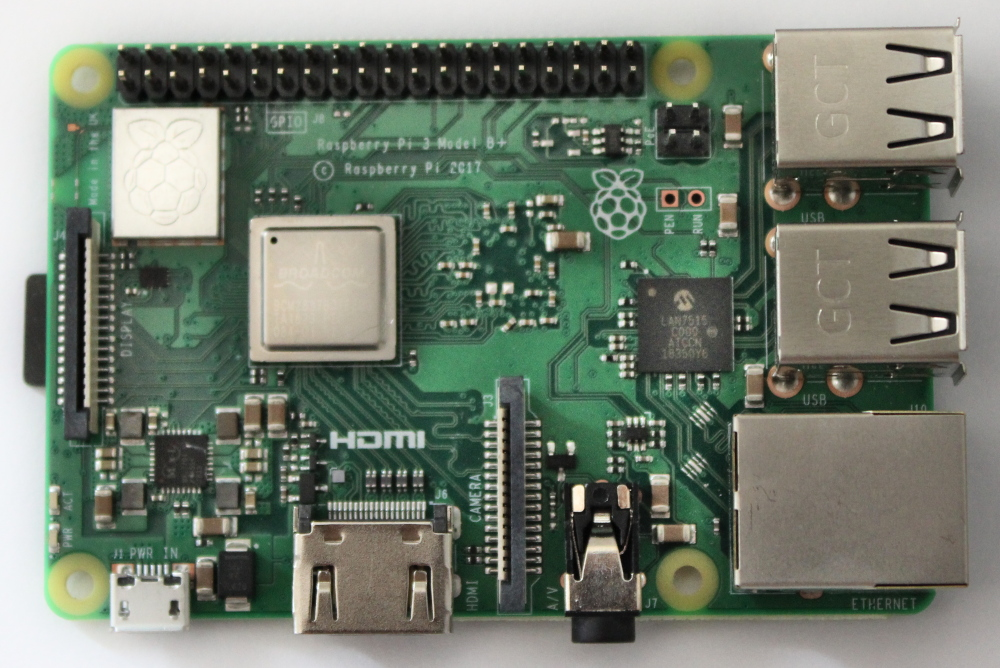
\includegraphics[width=.5\textwidth]{2-hardwaredesign/img/rasbperrypi_foto}
\end{center}

\bigskip
\teilaufgabe
Welche Signalarten liegen am J8-Header des Raspberry Pi an? Zählen Sie alle sieben,
in den Folien genannten Signalarten auf.


%-------------------------------------------------------------------------------
\aufgabe{Elektronik-Grundlagen}
%-------------------------------------------------------------------------------
\teilaufgabe
Innerhalb eines elektrischen Generators entsteht Strom, indem sich ein Magnet um
eine Drahtspule dreht. Das zugrunde liegende Prinzip nennt sich elektromagnetische
Induktion. Erklären Sie anhand folgender Abbildung, wie es dabei zum Stromfluss
kommt. Gehen Sie dabei auch kurz auf die Bestandteile des bohrschen Atommodells
ein, indem Sie die Grafik entsprechend beschriften.

\begin{center}
    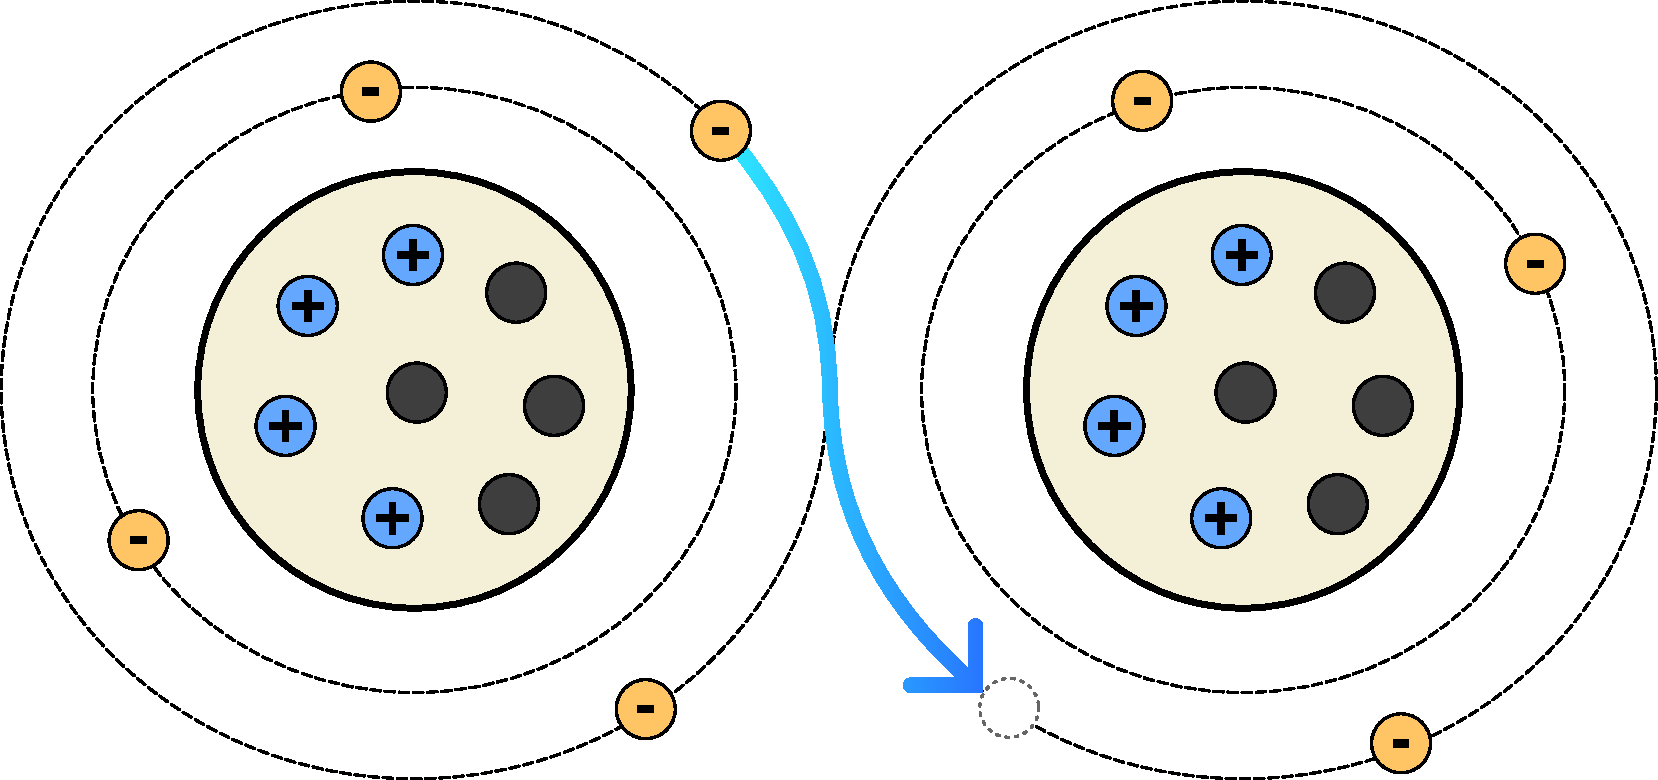
\includegraphics[width=.75\textwidth]{2-hardwaredesign/img/atom_elektronenfluss}
\end{center}

\bigskip
\teilaufgabe
Wann spricht man von einem Potential (auch Ladung) genannt und wann von einer
Spannung? Erklären Sie kurz, wie die beiden Begriffe zusammenhängen.

\bigskip
\teilaufgabe
Neben der Spannung sind Stromstärke, Widerstand und Leistung drei weitere
wichtige Größen der Elektrotechnik. In welchen Einheiten werden sie gemessen
und was drücken sie jeweils aus? Füllen Sie hierzu stichwortartig die folgende
Tabelle aus.

{
    \renewcommand{\arraystretch}{1.8}
    \medskip

    \begin{tabular}{|p{.15\textwidth}|p{.15\textwidth}|p{.7\textwidth}|}
        \hline
        \textbf{Kenngröße} & \textbf{Einheit} & \textbf{Bedeutung} \\
        \hline
        Spannung           &                  &                    \\[3em]
        \hline
        Stromstärke        &                  &                    \\[3em]
        \hline
        Leistung           &                  &                    \\[3em]
        \hline
        Widerstand         &                  &                    \\[3em]
        \hline
    \end{tabular}

    \medskip
}

\bigskip
\teilaufgabe
Die folgenden zwei Abbildungen zeigen, wie Spannung, Stromstärke, Widerstand
und Leistung gemäß dem ohmschen Gesetz in Zusammenhang stehen. Welche Größen
werden durch die jeweiligen Formelzeichen beschrieben und wie lauten die Formeln
hinter den Abbildungen?

\begin{center}
    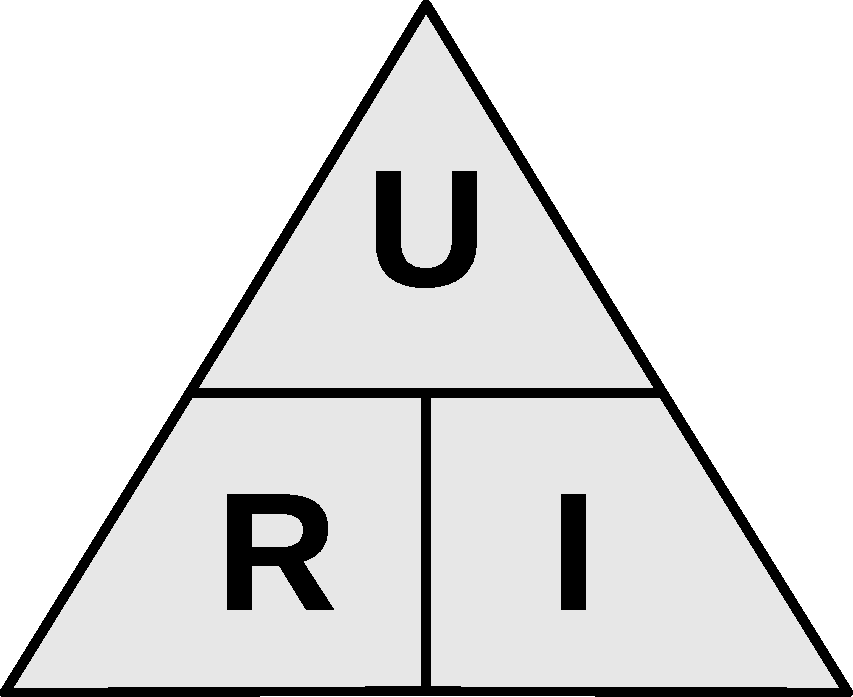
\includegraphics[width=3cm]{2-hardwaredesign/img/formel_uri}
    \hskip 3em
    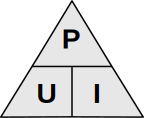
\includegraphics[width=3cm]{2-hardwaredesign/img/formel_pui}
\end{center}

\bigskip
\teilaufgabe
Berechnen Sie die gesuchten Werte für Widerstand, Stromstärke und Leistung in den
folgenden Anwendungsfällen:

\begin{enumerate}
    \item Die Spannung eines Ausgangspins am Rasbperry Pi beträgt 3,3\,V. Eine
    daran angeschlossene Leuchtdiode soll mit 2\,V und 5\,mA betrieben werden.
    Welcher Widerstand wird hierfür benötigt?

    \item Eine Eingangsspannung von 3,3\,V wird durch einen 1k\,\si{\ohm} Widerstand
    mit einem Eingangspin des Raspberry Pi verbunden. Welche Stromstärke fließt
    dabei?

    \item Ein typisches Netzteil für den Raspberry Pi funktioniert als
    Festspannungsnetzteil und liefert maximal 2\,A Strom bei 5\,V Spannung.
    Wie viel Watt verbraucht das Netzteil unter Volllast?
\end{enumerate}

%-------------------------------------------------------------------------------
\aufgabe{Spannungs- und Stromteiler}
%-------------------------------------------------------------------------------
\teilaufgabe
Gegeben sei eine einfache Schaltung mit drei in Reihe geschalteten Verbrauchern
und einem Steckernetzteil als Spannungsquelle. Angenommen, das Netzteil liefert
12\,V Spannung und die Verbraucher haben den Widerstand 910\,\si{\ohm}, 750\,\si{\ohm}
und 3k\,\si{\ohm}.

\begin{itemize}
    \item Welche Teilspannungen fallen an den einzelnen Verbrauchern ab?
    \item Wie hoch ist der Strom, der durch die Schaltung fließt?
    \item Wie viele Kilowattstunden fallen an, wenn die Schaltung 24 Stunden läuft?
\end{itemize}

\bigskip
\teilaufgabe
Angenommen, die oben genannten Verbraucher wären nicht in Reihe sondern parallel
geschaltet.

\begin{itemize}
    \item Welche Teilströme stehen den Verbrauchern dann zur Verfügung?
    \item Welcher Gesamtstrom fließt in diesem Fall durch die Schaltung?
    \item Wie hoch ist der Gesamtwiderstand der Schaltung?
\end{itemize}

\bigskip
\teilaufgabe
Angenommen, nur die Verbraucher zwei und drei mit den Widerständen 750\,\si{\ohm}
und 3k\,\si{\ohm} wären parallel geschaltet und der Verbraucher mit 910\,\si{\ohm}
wäre als Reihenschaltung davor angeordnet.

\begin{itemize}
    \item Wie teilt sich die Spannung zwischen den einzelnen Verbrauchern auf?
    \item Wie hoch ist der Gesamtwiderstand der Schaltung im Vergleich nun?
    \item Welcher Gesamtstrom fließt in diesem Fall durch die Schaltung?
\end{itemize}

%-------------------------------------------------------------------------------
\aufgabe{Digitale Komponenten verbinden}
%-------------------------------------------------------------------------------
\teilaufgabe
Im letzten Aufgabenblatt haben wir integrierte Schaltkreise mit \glqq{}Chip Enable\grqq{}
genannten Eingängen gesehen. Die anderen Ein- und Ausgänge der Bausteine müssen
daher so genannte \glqq{}Tri-States\grqq{} sein. Recherchieren Sie den Begriff
Tri-State und erklären Sie mit wenigen Worten, was damit gemeint ist und warum die
kennengelernte Schaltung ohne Tri-States nicht funktionieren würde.

\bigskip
\teilaufgabe
In den Folien wurde mit einem einfachen Spannungsteiler ein 5\,V-Sensorsignal
auf für den Raspberry Pi verträgliche 3,3\,V herunter geregelt. Für solche
Aufgaben wird allerdings eher selten ein Spannungsteiler verwendet, da er ein
paar entscheidende Nachteile besitzt:


\begin{enumerate}
    \item Die Schaltung verbraucht vergleichsweise viel Strom, der als überschüssige
    Energie durch die Widerstände in Wärme umgesetzt wird.

    \item Das Eingangssignal wird durch die Schaltung zeitlich verwischt, so dass
    nur eine begrenzte Datenrate übertragen werden kann.
\end{enumerate}

Entwerfen Sie daher eine Schaltung, die anstelle eines Spannungsteilers einen
Transistor nutzt, um den Eingangspin des Raspberry Pi mit 3,3\,V anzusteuern.
Begrenzen Sie dabei die maximal an den Pi abgegebene Strommenge auf 0,2\,mA.

\clearpage
\teilaufgabe
Wozu werden in einer digitalen Schaltung Pullup- oder Pulldown-Widerstände
genutzt. Erklären Sie kurz, wie die Widerstände verschaltet sind und welche
Aufgabe sie erfüllen.

\bigskip
\teilaufgabe
In einer Alarmanlage soll eine LED unterschiedlich schnell blinken, je nachdem
ob die Alarmanlage scharf geschaltet ist oder nicht. Im ausgeschalteten Zustand
soll die LED immer eine Sekunde lang an und eine halbe Sekunde lang aus sein.
Eingeschaltet soll sie jeweils nur eine halbe Sekunde lang an und aus sein.
Mit welchen Parametern müsste ein pulsweitenmodulierter Ausgang des Raspberry
Pi konfiguriert werden, um diese Zeitintervalle zu erreichen?

%-------------------------------------------------------------------------------
\aufgabe{Serielle Datenübertragung}
%-------------------------------------------------------------------------------
\teilaufgabe
Die Kommunikation innerhalb eines eingebetteten Systems erfolgt oftmals über
serielle Schnittstellen. Und wie nicht anders zu erwarten, haben unterschiedliche
Hersteller unterschiedliche, zueinander inkompatible Standards hierfür geschaffen.
Füllen Sie die nachfolgende Tabelle mit den Eigenschaften der wichtigsten vier
Standards aus:

\newcommand{\SerialVergleich}[1]{
    {
        \renewcommand{\arraystretch}{1.8}
        \newcolumntype{Y}{>{\centering\arraybackslash}X}
        \newcolumntype{R}{>{\raggedleft\arraybackslash}p}
        \vskip \LTpre

        \begin{tabularx}{\textwidth}{|R{.33\textwidth}|X|X|X|X|}
            \hline
            &
            \textbf{UART}    &
            \textbf{SPI}     &
            \textbf{I²C}     &
            \textbf{1-wirte}
            \\

            \hline
            \textbf{Synchron / Asynchron} &
            \loesungswert{#1}{...} &        % URART
            \loesungswert{#1}{...} &        % SPI
            \loesungswert{#1}{...} &        % I²C
            \loesungswert{#1}{...}          % 1-wire
            \\[2em]

            \hline
            \textbf{Full-Duplex, Half-Duplex} &
            \loesungswert{#1}{...} &        % URART
            \loesungswert{#1}{...} &        % SPI
            \loesungswert{#1}{...} &        % I²C
            \loesungswert{#1}{...}          % 1-wirte
            \\[2em]

            \hline
            \textbf{Mehrere Empfänger möglich} &
            \loesungswert{#1}{...} &        % URART
            \loesungswert{#1}{...} &        % SPI
            \loesungswert{#1}{...} &        % I²C
            \loesungswert{#1}{...}          % 1-wirte
            \\[2em]

            \hline
            \textbf{Mehrere Sender möglich} &
            \loesungswert{#1}{...} &        % URART
            \loesungswert{#1}{...} &        % SPI
            \loesungswert{#1}{...} &        % I²C
            \loesungswert{#1}{...}          % 1-wirte
            \\[2em]

            \hline
            \textbf{Adressierung der Empfänger} &
            \loesungswert{#1}{...} &        % URART
            \loesungswert{#1}{...} &        % SPI
            \loesungswert{#1}{...} &        % I²C
            \loesungswert{#1}{...}          % 1-wirte
            \\[2em]

            \hline
        \end{tabularx}

        \vskip \LTpost
    }
}
\SerialVergleich{}

\bigskip
\teilaufgabe
Ein über SPI angebundener Temperatursensor sendet immer genau zwei Bytes für
einen Temperaturwert. Das erste Byte entspricht dabei der Temperatur in Grad
Celsius ohne Nachkommastellen, das zweite Byte liefert die Zahl hinter dem Komma.
Zeichnen Sie ein Timingdiagramm, aus dem der zeitliche Ablauf aller Signale
hervorgeht, wenn der Sensor den Wert 28.3 liefert.

% Übungsstunde: Entwurf einer Alarmanlage
%  » Bewegungssensor zur Aktivierung der Alarmanlage
%  » LCD-Display zur Ausgabe einer Eingabeaufforderung
%  » Knöpfe zur Eingabe des Deaktivierungscodes
%  » Kamera zum Aufnehmen von Fotos
%  » Vorgegebenes Node-RED-Programm zum Auslösen eines Alarams per E-Mail



%===============================================================================
\clearpage
\LoesungHeader
%===============================================================================

%-------------------------------------------------------------------------------
\loesung{Kontakt zur Außenwelt}
%-------------------------------------------------------------------------------
\teilaufgabe
Die vier Abstraktionsebenen im Hardwaredesign, jeweils mit zwei Vor- und
Nachteilen:

\begin{enumerate}
    %%
    \item \textbf{Elementare Bauteile} \\
    Widerstände, Transistoren, Dioden, Relais, Leuchtdioden, Taster, Schalter, ...

    {
        \small
        Vorteile:

        \begin{compactitem}
            \item Exakt auf den Anwendungsfall zugeschnittene Schaltungen realisierbar
            \item Minimale Kosten durch minimale Anzahl an Zusatzkomponenten
        \end{compactitem}

        Nachteile:

        \begin{compactitem}
            \item Hardwaredesign und Interfacing vergleichsweise aufwändig
            \item Fertigung dauerhaft einsetzbarer Schaltungen ebenfalls aufwändig
        \end{compactitem}
    }

    \smallskip

    %%
    \item \textbf{Integrierte Schaltkreise} \\
    Mikrocontroller, Speicherbausteine, Logikbausteine, Level Shifter, ...

        {
        \small
        Vorteile:

        \begin{compactitem}
            \item Deutliche Miniaturisierung und Vereinfachung komplexer Schaltungen
            \item Einfacheres Hardwaredesign dank vieler verfügbarer Standardkomponenten
        \end{compactitem}

        Nachteile:

        \begin{compactitem}
            \item Extrem große Auswahl und daher aufwändige Recherchen erforderlich
            \item Immer weniger DIL-Komponenten, die sich einfach verlöten lassen
        \end{compactitem}
    }

    \smallskip

    %%
    \item \textbf{Vorgefertigte Baugruppen} \\
    RFID-Leser, Kameramodule, LCD-Displays, Sensormodule, Folientastaturen, ...

    {
        \small
        Vorteile:

        \begin{compactitem}
            \item Baukastenprinzip zur Realisierung komplexer Hardwaredesigns
            \item Interfacing daher bereits mit sehr einfachen Schaltungen möglich
        \end{compactitem}

        Nachteile:

        \begin{compactitem}
            \item Vergleichsweise hohe Kosten gegenüber den zugrunde liegenden Bauteilen
            \item Komponenten unterschiedlicher Hersteller oft inkompatibel zueinander
        \end{compactitem}
    }

    \smallskip

    %%
    \item \textbf{Modulare Geräte} \\
    IP-Kameras, USB-Lautsprecher, Industriesteuergeräte, ZigBee-Komponenten, ...

        {
        \small
        Vorteile:

        \begin{compactitem}
            \item So gut wie keine Hardwarekenntnisse erforderlich
            \item Nutzung von Off-the-Shelve PC-Komponenten möglich
        \end{compactitem}

        Nachteile:

        \begin{compactitem}
            \item Sehr viel teurer als alle anderen Varianten
            \item Deutlich höhere Gesamtkomplexität des Systems
        \end{compactitem}
    }
\end{enumerate}

\clearpage
\teilaufgabe
Beschriftung der Hardwareschnittstellen des Raspberry Pi:

\begin{center}
    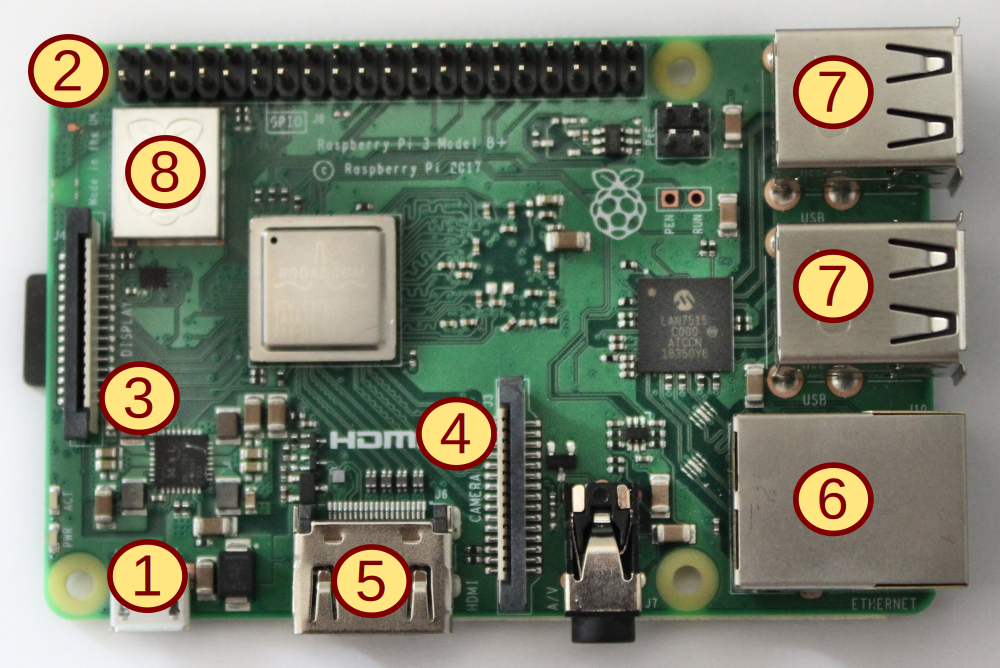
\includegraphics[width=.5\textwidth]{2-hardwaredesign/img/raspberry_anschluesse}
\end{center}

\begin{tabularx}{\textwidth}{XX}
        1. Mini-USB-Stromversorgung     &   5. HDMI-Bildschirmanschluss     \\
        2. J8 GPIO-Header               &   6. LAN-Netzwerkanschluss        \\
        3. Display Serial Interface     &   7. USB-Anschlüsse               \\
        4. Camera Serial Interface      &   8. WiFi, Bluetooth              \\
\end{tabularx}

\bigskip
\teilaufgabe
Signalarten am J8-Header des Raspberry Pi:

\medskip

\begin{tabularx}{\textwidth}{XX}
    \textbf{Stromversorgung:}   &   \textbf{Digital Ein-/Ausgänge:}     \\
    5\,V Power                  &   GPIO                                \\
    3.3\,V Power                &   Pulsweitenmodulation                \\
    Ground (Masse)              &   Asynchron serielle Schnittstellen   \\
                                &   Synchron serielle Schnittstellen    \\
\end{tabularx}

%-------------------------------------------------------------------------------
\loesung{Elektronik-Grundlagen}
%-------------------------------------------------------------------------------
\teilaufgabe
In der Abbildung gezeigte Bestandteile des bohrschen Atommodells:

\smallskip

\includegraphics[width=.5cm]{2-hardwaredesign/img/atom_kern}      Atomkern  \hskip 2em
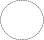
\includegraphics[width=.5cm]{2-hardwaredesign/img/atom_schale}    Schale    \hskip 2em

\includegraphics[width=.5cm]{2-hardwaredesign/img/atom_elektron}  Elektron  \hskip 2em

\includegraphics[width=.5cm]{2-hardwaredesign/img/atom_proton}    Proton    \hskip 2em

\includegraphics[width=.5cm]{2-hardwaredesign/img/atom_neutron}   Neutron

Laut dem bohrschen Atommodell besteht ein Atom aus einem Kern mit positiv geladenen
Protonen und neutralen Neutronen, um den in mehreren Bahnen (auch Schalen genannt)
negativ geladene Neutronen kreisen. Im Normalzustand besitzt das Atom dabei genauso
viele Elektronen wie Protonen. Die durch das sich drehende, magnetische Feld erzeugte
Lorentzkraft versetzt die Elektronen der äußeren Bahn (die sogenannten Valenzelektronen)
in Bewegung und sorgt so dafür, dass sie auf benachbarte Atome überspringen. Die Richtung
wird dabei durch die Bewegung des Magnetfelds vorgegeben, so dass dadurch eine gerichtete
Bewegung der Elektronen durch das leitende Material und somit ein Stromfluss entstehen.

\bigskip
\teilaufgabe
Potential oder Ladung bezeichnen den atomaren Zustand des Elektronenüberschusses
oder Elektronenmangels. Da Elektronen per Definition negativ geladen sind, besitzt
ein Atom mit zu wenigen Elektronen eine positive Ladung, da es mehr positive als
negative Ladungsträger besitzt. Umgekehrt besitzt ein Atom mit mehr Elektronen als
Protonen eine negative Ladung. Die dazugehörige Maßeinheit nennt sich Coulumb.

Die Ladung oder das Potential werden immer an einem Punkt gemessen und beziehen
sich auf den Normalzustand, indem ein Atom genauso viele Elektronen wie Protonen
besitzt und somit elektrisch neutral ist. Eine Spannung wird hingegen immer zwischen
zwei Punkten gemessen, da es sich dabei um die Ladungsdifferenz zwischen den beiden
Punkten handelt. Diese Ladungsdifferenz ist die Voraussetzung dafür, dass Strom
fließen kann, wenn die beiden Punkte über ein leitfähiges Material verbunden werden.


\bigskip
\teilaufgabe
Wichtige Bezugsgrößen der Elektrotechnik:

{
    \renewcommand{\arraystretch}{1.8}
    \medskip

    \begin{tabular}{|p{.15\textwidth}|p{.15\textwidth}|p{.7\textwidth}|}
        \hline
        \textbf{Kenngröße} &
        \textbf{Einheit}   &
        \textbf{Bedeutung} \\

        \hline
        Spannung &
        Volt &
        Beschreibt die Ladungsdifferenz zwischen zwei Punkten, vergleichbar mit
        dem Druck, den eine Pumpe auf das Wasser in einem Wasserschlauch ausübt.
        \\

        \hline
        Stromstärke &
        Ampere &
        Beschreibt wie viele Elektronen in einer gegebenen Zeit fließen, vergleichbar
        mit der Menge und Geschwindigkeit, mit der Wasser durch einen Schlauch fließt.
        \\

        \hline
        Leistung &
        Watt &
        Beschreibt die in einer Zeiteinheit verrichtete Arbeit bzw. umgesetzte Energie.
        Da der Zeitquotient bereits in der Formel für die Stromstärke enthalten ist,
        kann die Leistung einfach als Produkt aus Spannung und Strom berechnet werden.
        \\

        \hline
        Widerstand &
        Ohm &
        Ein Widerstand hindert die Bewegung der Elektronen und legt somit bei
        gegebener Spannung die erzielte Stromstärke fest. Hierfür setzt er einen
        Teil des Stroms in thermische Energie um und \glqq{}vernichtet\grqq{}
        ihn sozusagen.
        \\

        \hline
    \end{tabular}

    \medskip
}

\bigskip
\teilaufgabe
Formelzeichen für die wichtigsten Berechnungen:

\textbf{U} = Spannung
\hskip 2em
\textbf{I} = Stromstärke
\hskip 2em
\textbf{R} = Widerstand
\hskip 2em
\textbf{P} = Leistung

Dazugehörige Formeln:

$U = R / I$
\hskip 2em
$R = U / I$
\hskip 2em
$I = U / R$
\hskip 6em
$P = U * I$
\hskip 2em
$U = P / I$
\hskip 2em
$I = P / U$

\bigskip
\teilaufgabe
Berechnung von Widerstand, Stromstärke und Leistung:

\begin{enumerate}
    %%
    \item Da der Raspberry Pi 3,3\,V liefert, die LED aber nur 2\,V verträgt,
    muss der gesuchte Widerstand die Differenz von 1,3\,V \glqq{}vernichten\grqq{}:

    $
        U_{Pi} = 3,3\,V \\
        U_{LED} = 2\,V \\
        \smallskip
        U_{Zuviel} = U_{Pi} - U_{LED} = 1,3\,V
    $

    Dieser Wert lässt sich nun mit der gewünschten Stromstärke von 5\,mA verwenden,
    um den Widerstandswert zu berechnen:

    $
        I_{LED} = 5\,mA \\
        \smallskip
        R = U_{Zuviel} / I_{LED} = 1,3\,V / 0,005\,A = 260\,\si{\ohm}
    $

    \textbf{Hinweis:} 260\,\si{\ohm} liegen genau zwischen den in der Widerstandsreihe
    E24 verfügbaren Widerständen 240\,\si{\ohm} und 270\,\si{\ohm}. In der Praxis
    würde man daher einfach den nächst höheren Widerstand von 270\,\si{\ohm} verwenden
    und prüfen, ob die LED auch mit dem etwas geringeren Strom arbeitet.

    %%
    \item Gemäß der Gleichung $I = U / R$ fließen $3,3\,V / 1000\,\si{\ohm} = 3,3\,mA$.

    %%
    \item Gemäß der Gleichung $P = U * I$ bestizt das Netzeil eine Leistung von
    $5\,V * 2\,A = 10\,W$.

    \textbf{Hinweis:} Läuft das Netzteil daher eine Stunde unter Vollast, entstehen
    dadurch 0,01\,kWh (Kilowattstunden) Stromkosten.
\end{enumerate}

%-------------------------------------------------------------------------------
\loesung{Spannungs- und Stromteiler}
%-------------------------------------------------------------------------------
Wird nachgereicht!

%-------------------------------------------------------------------------------
\loesung{Digitale Komponenten verbinden}
%-------------------------------------------------------------------------------
Wird nachgereicht!

%-------------------------------------------------------------------------------
\loesung{Serielle Datenübertragung}
%-------------------------------------------------------------------------------
Wird nachgereicht!
